\chapter{CMS Experiment at LHC}
\section*{Large Hadron Collider (LHC)}
\begin{wrapfigure}{l}{0.4\textwidth}
    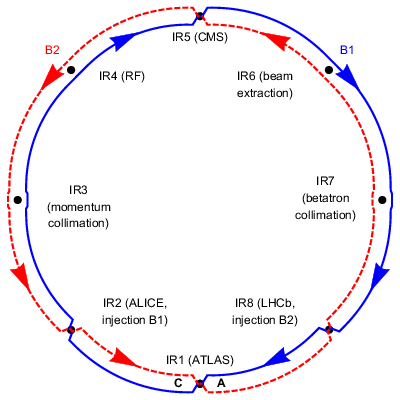
\includegraphics[width=0.4\textwidth]{LHC.png}
    \caption{Schematic view of the LHC and the interaction points}
    \label{Fig:LHC}
\end{wrapfigure}
The Large Hadron Collider (LHC) is a  two-ring hadron accelerator and collider, located at the European Organization for Nuclear Research (CERN) in Geneva, Switzerland. The LHC consists of a 27-kilometer circular tunnel situated 100 meters below ground level and is designed to collide proton beams at a center-of-mass energy of 14TeV, as well as collide heavy ion beams. The beams are accelerated trough the magnetic field of superconducting electromagnet in opposite directions in separate beam pipes and crossed at four interaction points as shown in Fig. \ref{Fig:LHC}. The detectors located at these interaction points (IPs) are designed to study the products of pp collisions. The four experiments performed at these interaction points are as follows: The ATLAS (A Toroidal LHC ApparatuS) Experiment at IP1, and The CMS (Compact Muon Solenoid) Experiment at IP5 are general purpose detectors designed to detect a broad range of particles generated in pp collisions or heavy-ion collisions at the highest collision rates of the LHC. The ALICE (A Large Ion Collider Experiment) Experiment at IP1 is designed to investigate the properties of quarks and gluons at extreme energy densities, and The LHCb Experiment at IP8 is designed to study B meson related physics.\\
\\
The process of accelerating protons in the LHC involves several steps. First, the protons, hydrogen gas stripped of its electrons, are accelerated to an energy of 50 MeV in a Linear Accelarator (LINAC). After leaving the LINAC in bunches of protons, they enter the Proton Synchrotron Booster (PSB), where they are further accelerated to an energy of 1.4 GeV. Next, the proton bunches enter the Proton Synchrotron (PS), where they are accelerated to an energy of 25 GeV. Finally, the protons are injected into the Super Proton Synchrotron (SPS), where they are accelerated to an energy of 450 GeV. Once the protons reach their final energy of 450 GeV in the SPS, they are transferred to the LHC, where they are further accelerated to their maximum energy.

The LHC has had several runs since it began operations in 2009. "Run 1" was the first operational run of the LHC, which began in 2009 and lasted until 2013. During this run, the LHC collided protons at a center-of-mass energies of up to 8 TeV, which led to the discovery of the Higgs boson in 2012. After a long shutdown for upgrades on the LHC and detectors, the LHC continued operations of pp collisions in 2015 at an increased center-of-mass energy of 13 TeV. "Run 3' Data-taking took place until shutdown at the end of 2018 . ATLAS and CMS obtaining a total of 140$fb^{-1}$ integrated luminosity of pp collision data over the four years for physics analysis.